\chapter{Estado da Arte}
\label{chap:estado-da-arte}

\section{Enquadramento Teórico} \label{sec:background}

Esta secção serve como base teórica para clarificar alguns conceitos importantes para o projeto, permitindo uma melhor compreensão das secções que se seguem.\\\par

%%In this section, you should describe the scientific or technological context of your project. Provide enough information so that a reader unfamiliar with the topic can understand the problem you are addressing and the rationale for your project. This may include relevant concepts and definitions in the area, particularly those that will be used throughout this document.

\subsection{Geração automática de código}
\noindent{A} geração automática de código consiste na produção de código fonte a partir de descrições de alto nível, como requisitos em linguagem natural, modelos formais ou representações estruturadas, com o objetivo de acelerar o desenvolvimento e reduzir tarefas repetitivas.\par

\medskip\noindent{Apesar} da geração automática de código estar hoje em dia associada à inteligência artificial generativa, a ideia não é nova. Abordagens como o Model-Driven Engineering (MDE)\cite{MDE-Schmidt,MDEInPratice} e as linguagens específicas de domínio (DSLs)\cite{DSLs} já permitiam gerar código a partir de modelos formais ou descrições declarativas. No entanto, estas técnicas assentam em regras rígidas e gramáticas estritamente definidas, sendo eficazes sobretudo em domínios controlados e pouco flexíveis perante requisitos abertos ou em linguagem natural.\\\par

\noindent{Os} modelos de IA generativa, amplamente disponibilizados a partir de 2022, marcaram uma evolução na geração automática de código ao permitirem interpretar instruções pouco estruturadas em linguagem natural\cite{Codex}. Esta capacidade resulta do treino em grandes volumes de dados heterogéneos, que combinam linguagem natural e código fonte, permitindo aprender padrões sintáticos e relações entre componentes de programas.\\

\noindent{Uma} parte importante desta evolução deve-se à arquitetura \textit{Transformer}, proposta em 2017 por Vaswani et al.\cite{Transformer}. Os \textit{Transformers} utilizam mecanismos de atenção que relacionam tokens distantes numa sequência, capturando dependências de longo alcance e identificando as partes mais relevantes da instrução, o que se revelou altamente eficiente para tarefas de linguagem natural e permitiu treinar modelos de grande escala capazes de gerar código coerente\cite{Codex}.\\

%%\begin{figure}[htbp]
  %%  \centering
  %%  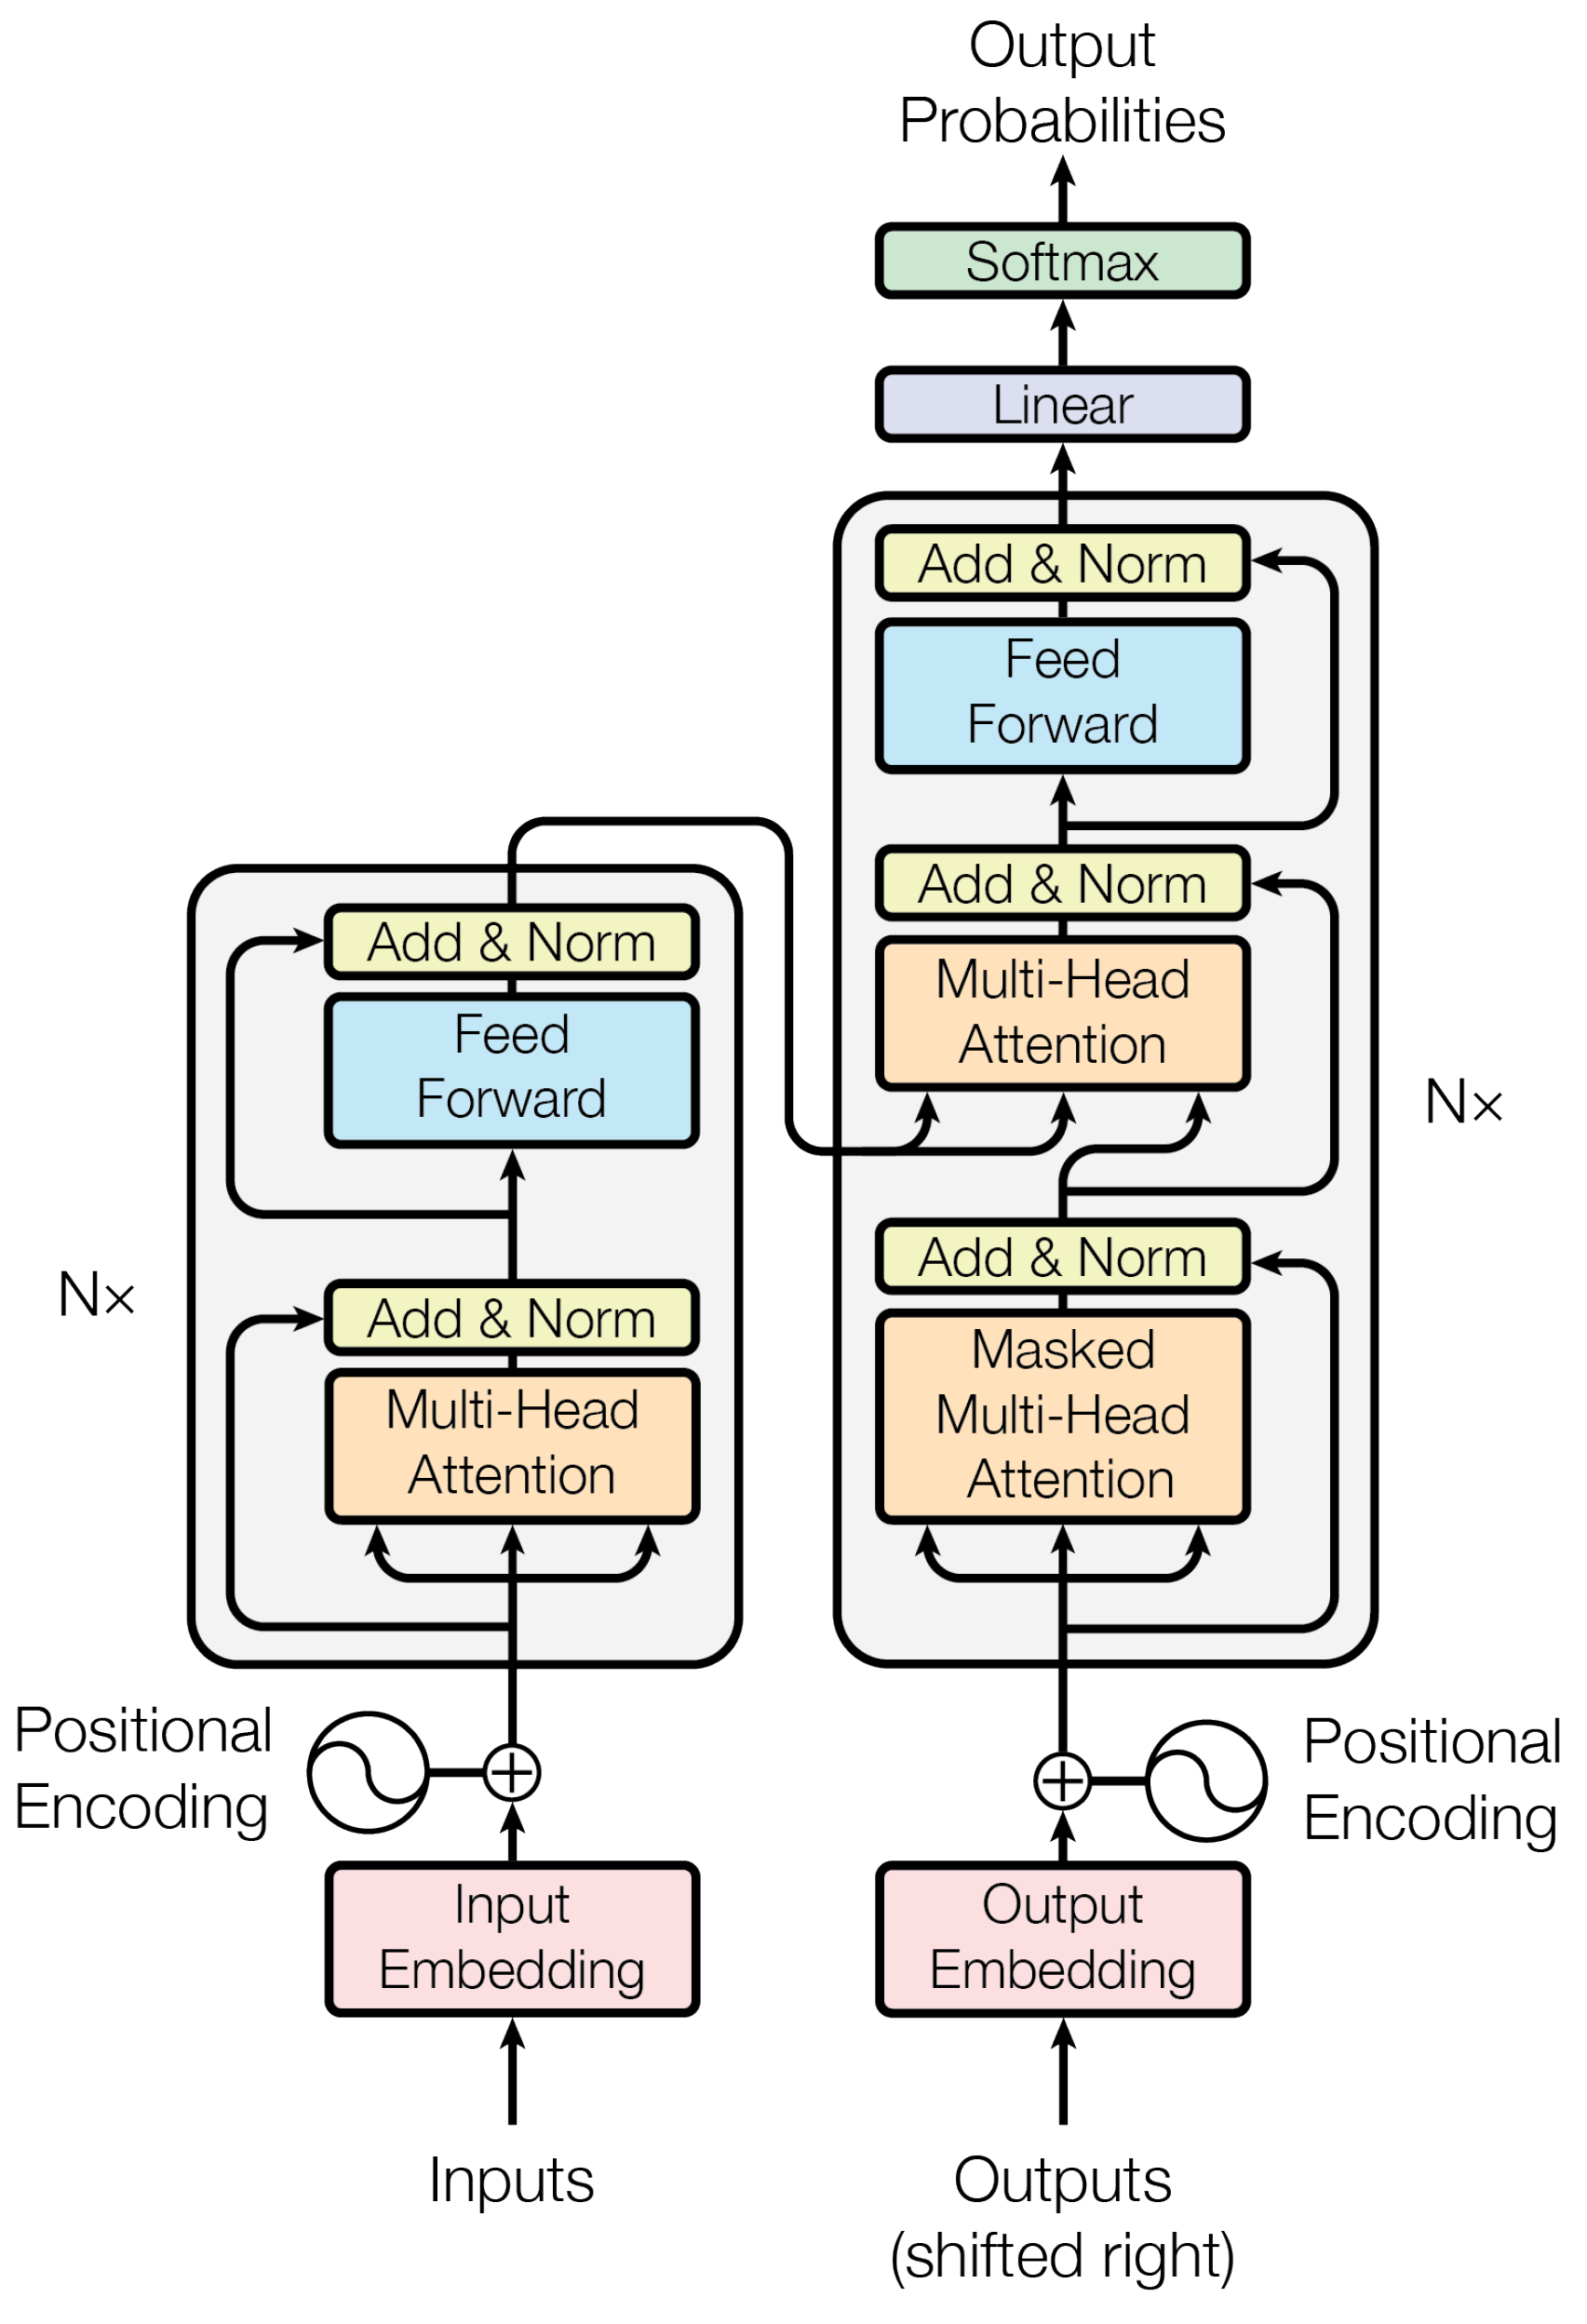
\includegraphics[height=0.4\textheight, width=0.3\textwidth]{../img/transformer.png}
  %%  \caption{Arquitetura Transformer proposta por Vaswani et al.\cite{Transformer}}
  %%  \label{fig:transformer}
%%\end{figure}

\noindent{Nos} últimos anos têm surgido diversos sistemas que exploram modelos de linguagem para apoiar ou automatizar partes do desenvolvimento de software, recorrendo a modelos únicos ou a combinações de etapas especializadas para orientar e validar a geração. Esta diversidade reflete a maturidade crescente da área e o interesse em integrar LLMs como assistentes ativos no fluxo de trabalho do programador. Exemplos representativos são discutidos na secção \ref{CODE_GENERATION_TR}.\\\par

\subsection{Ciclo de Vida do Desenvolvimento de Software}

\noindent{Apesar} do potencial das LLMs na geração de código, a construção de um produto de software envolve um conjunto mais amplo de fases, cuja natureza e formalização variam consoante o contexto organizacional. Para contextualizar o papel da automatização, é necessário compreender o ciclo de vida do desenvolvimento de software\cite{ALLLIFECYCLE} e identificar as etapas onde esta pode ser introduzida.\\\par

\noindent{Estas} etapas incluem, em primeiro lugar, o levantamento e análise de requisitos, que visam garantir que as necessidades do cliente sejam adequadamente compreendidas, estruturadas e documentadas. O processo de levantamento de requisitos envolve diversas técnicas, incluindo entrevistas e revisões literárias, como evidenciado por Lim et al.\cite{RE}, que destacam a importância de métodos eficazes para alcançar uma compreensão abrangente das necessidades dos utilizadores, uma vez que os requisitos devidamente capturados constituem a base sobre a qual todo o ciclo de vida do software é construído.\par

\noindent{Com} os requisitos definidos, a modelação funcional e estrutural do sistema surge como etapa subsequente, frequentemente suportada por linguagens formais e semi-formais de representação como a UML (Unified Modeling Language), BPMN (Business Process Model and Notation) para processos de negócio ou SysML (Systems Modeling Language) para sistemas complexos. Estas linguagens permitem traduzir requisitos textuais em representações visuais, facilitando a análise, validação e comunicação entre equipas técnicas e não técnicas. Os modelos UML desempenham um papel crítico na documentação e validação de requisitos, servindo como elementos centrais de coordenação entre diferentes perspetivas do sistema\cite{UML}. Esta modelação inclui diagramas de casos de uso, classes, atividades ou sequência, que complementam a descrição funcional do sistema e ajudam a desenhar o comportamento desejado. Neste contexto, a conceção de interfaces e fluxos de interação emerge como um artefacto fundamental, permitindo validar o comportamento esperado do sistema do ponto de vista do utilizador e servindo de base para decisões técnicas posteriores, nomeadamente ao nível da definição de APIs e da implementação.\par

\noindent{A} definição de APIs (Application Programming Interfaces) e dos componentes arquiteturais constitui outra etapa fundamental, pois estabelece os contratos de comunicação entre as diferentes partes do sistema. Especificações claras de APIs permitem uma implementação mais consistente, facilitam a integração entre módulos e suportam estratégias de teste orientadas a componentes e serviços.

\noindent{Depois} da definição dos componentes e das interfaces do sistema, segue-se a fase de implementação, onde o código é desenvolvido de acordo com as especificações definidas. Esta etapa envolve não apenas a programação propriamente dita, mas também a integração de módulos e a resolução de dependências técnicas, garantindo que os componentes funcionem de forma coesa. A implementação é acompanhada por atividades de verificação e validação, onde se aplicam diferentes níveis de testes, com o objetivo de identificar defeitos, avaliar comportamentos e assegurar que o software cumpre os requisitos estabelecidos. Por fim, a documentação técnica desempenha um papel transversal a todas estas fases, registando decisões, especificações, arquiteturas, APIs e procedimentos de utilização, facilitando a manutenção futura e promovendo uma compreensão consistente do sistema entre programadores e \textit{stakeholders}.\\\par

\noindent{Para} além das etapas que compõem o desenvolvimento de software, importa considerar também as metodologias que organizam estas atividades ao longo do ciclo de vida. Os processos tradicionais, como o modelo em cascata (Waterfall)\cite{Waterfall}, estruturavam o desenvolvimento de forma sequencial, com transições rígidas entre etapas. Com o tempo, esta abordagem revelou limitações em cenários de requisitos dinâmicos, particularmente em contextos de mudança frequente ou incerteza elevada, conduzindo à adoção de metodologias ágeis, que promovem ciclos iterativos, entregas incrementais e adaptação contínua às necessidades do utilizador\cite{Agile}, como ilustrado na Figura \ref{fig:waterfall_agile}.\\\par

\begin{figure}[htbp]
    \centering
    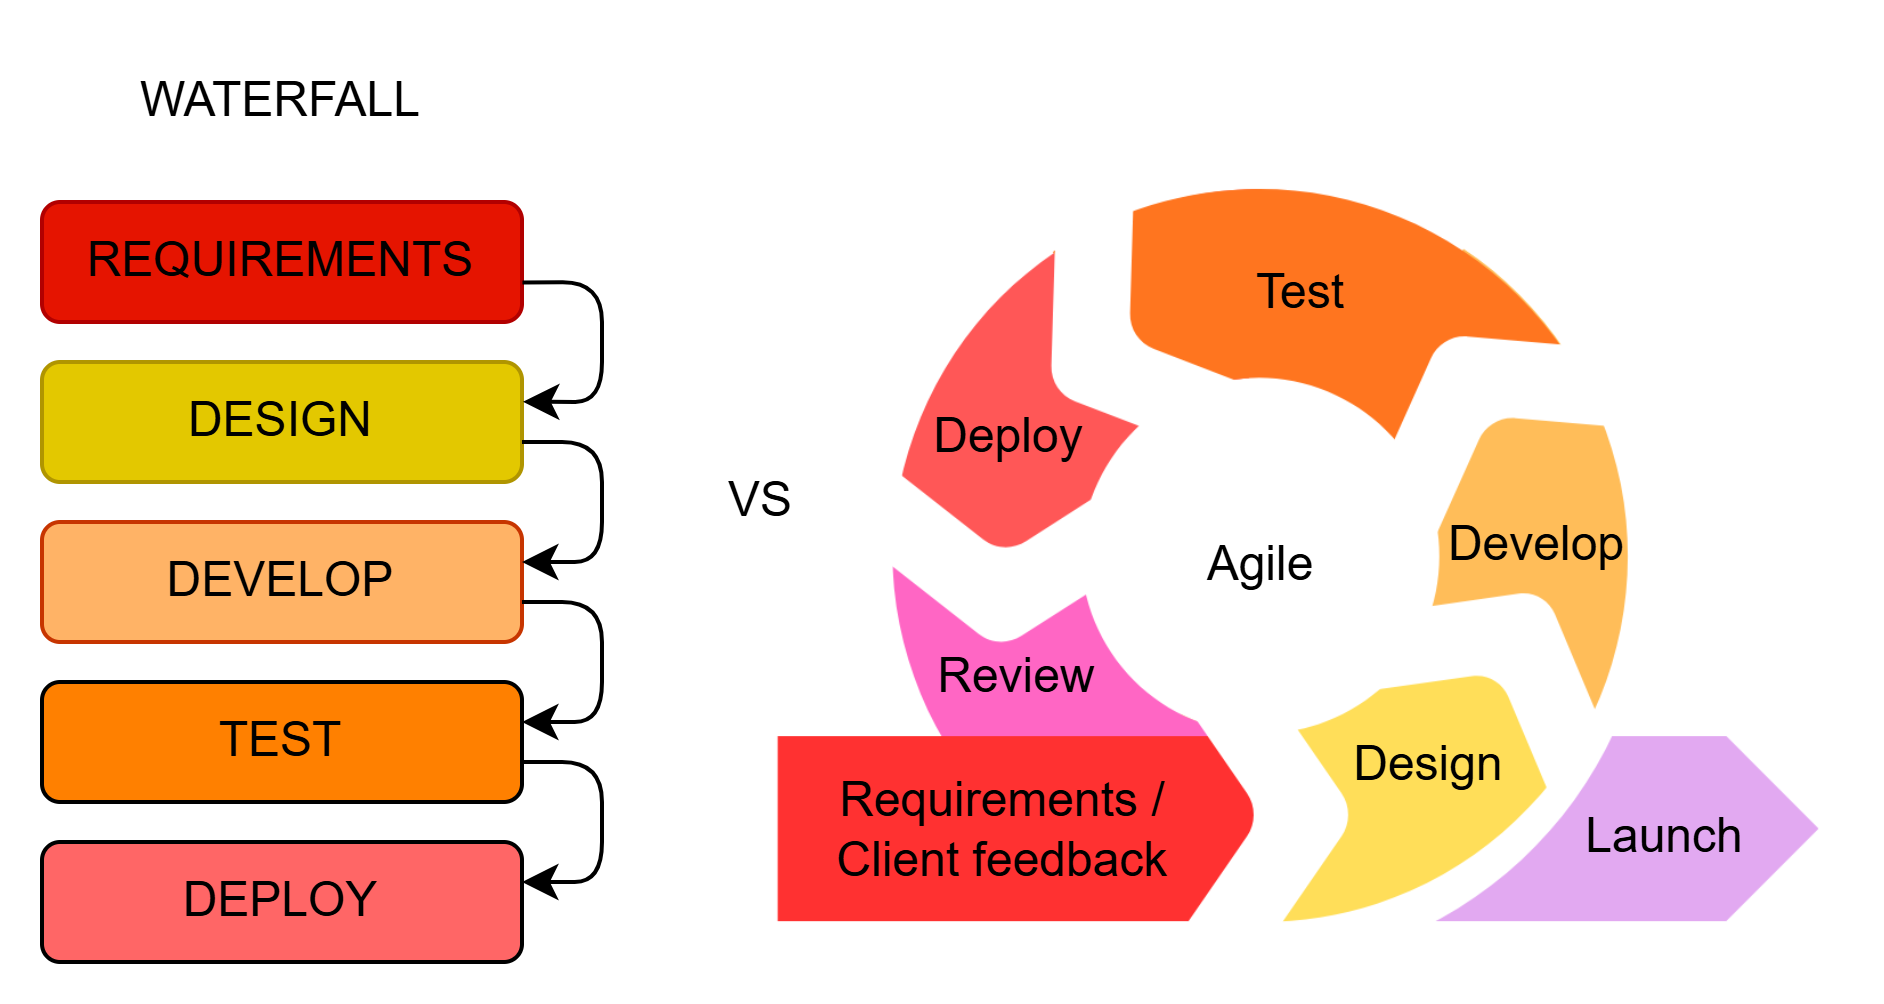
\includegraphics[height=0.2\textheight, width=0.45\textwidth]{../img/waterfall_agille.png}
    \caption{Comparação entre os modelos Waterfall e modelos Iterativos}
    \label{fig:waterfall_agile}
\end{figure}

\subsection{Limitações dos LLMs e Técnicas de Refinamento}
\label{PE-BACKGROUND}

\noindent{Apesar} dos avanços dos LLMs, estes modelos apresentam limitações relevantes, como a geração de código incorreto ou incompleto, inconsistências lógicas, alucinações factuais e dificuldades na interpretação de requisitos ambíguos. Estas limitações decorrem, em grande parte, da natureza estatística dos modelos e da ausência de mecanismos internos de verificação semântica.\par

\noindent{Uma} abordagem para mitigar estas limitações consiste no \textit{fine-tuning} com dados específicos de domínio, com o objetivo de ajustar o comportamento do modelo às necessidades de uma organização ou tarefa concreta. No entanto, esta estratégia implica custos elevados, sobretudo no caso de modelos de grande escala. Cottier et al.\cite{CostIncreaseInLLMS} demonstram que os custos computacionais associados ao treino e re-treino de LLMs têm aumentado de forma acentuada, com um crescimento médio de 2.4 vezes por ano desde 2016.\\\par

\noindent{Neste} contexto, a engenharia de prompts (\textit{prompt engineering}) tornou-se uma alternativa particularmente relevante, fornecendo técnicas que procuram otimizar as instruções fornecidas ao modelo, estruturando-as de modo a orientar o comportamento do LLM sem necessidade de treino adicional. Estudos recentes têm demonstrado que a forma como o prompt é construído influencia significativamente a qualidade do código gerado, a clareza das explicações e a capacidade de o modelo seguir passos complexos\cite{CopilotStudy}. Ao estabelecer padrões, estratégias e boas práticas de formulação de prompts\cite{PEinLLMS}, é possível alcançar resultados mais fiáveis e reduzir ambiguidades inerentes à interpretação do modelo. Para além destas boas práticas gerais, a literatura identifica ainda um conjunto variado de técnicas específicas, cada uma concebida para atingir objetivos distintos, desde a melhoria do raciocínio e lógica do modelo, até à redução de alucinações, conforme sistematizado por Sahoo et al.\cite{PETechniques}.\par

\noindent{Dado} que esta dissertação visa explorar a automatização de diferentes etapas do desenvolvimento de software, a engenharia de prompts assume um papel central enquanto mecanismo de controlo e refinamento do comportamento dos modelos utilizados. O baixo custo operacional e a ausência de necessidade de treino especializado tornam esta abordagem particularmente adequada ao contexto estudado, permitindo adaptar modelos generalistas às tarefas específicas que compõem a pipeline de geração de software.\par

\subsection{Ferramentas de Orquestração de Fluxos} \label{sec:ferramentas-orquestracao}

No contexto deste trabalho, a automatização de etapas do processo de desenvolvimento de software implica a coordenação de múltiplos modelos de linguagem, cada um responsável por uma fase distinta da pipeline. Para suportar esta coordenação de forma estruturada e controlada, torna-se necessário recorrer a ferramentas de orquestração que abstraiam a complexidade associada à gestão dos fluxos de geração, ao encadeamento de chamadas a diferentes modelos e à integração de mecanismos de validação e refinamento iterativo.

\noindent{Estas} plataformas funcionam como camada de controlo central da pipeline, permitindo estruturar o processo em componentes independentes e reutilizáveis. Cada componente pode encapsular uma tarefa específica, como a invocação de um modelo, o processamento de uma resposta ou a aplicação de uma regra de validação, sendo depois interligado com os restantes de forma a produzir um fluxo coerente e rastreável. Esta natureza modular facilita não só o desenvolvimento iterativo da solução, como também a sua manutenção e evolução ao longo do tempo.

\noindent{Uma} característica comum a estas plataformas é a sua capacidade de integração com múltiplos fornecedores de modelos de linguagem, o que permite selecionar o modelo mais adequado para cada tarefa específica sem alterar a arquitetura global da pipeline. No panorama atual, o Dify\footnote{\href{https://dify.ai}{https://dify.ai}}, o LangFlow\footnote{\href{https://www.langflow.org}{https://www.langflow.org}}, o Flowise\footnote{\href{https://flowiseai.com}{https://flowiseai.com}} e o n8n\footnote{\href{https://n8n.io}{https://n8n.io}} são exemplos representativos destas plataformas. Todas disponibilizam ambientes visuais e programáticos para a composição modular de pipelines baseadas em LLMs, suportam integração com múltiplos fornecedores de modelos e permitem incorporar lógica personalizada e mecanismos de validação ao longo do fluxo de geração.

\section{Trabalho Relacionado} \label{sec:relatedwork}

A presente secção reúne o estado da arte relevante para esta tese, apresentando trabalhos, modelos e ferramentas que abordam problemas relacionados com a aplicação de métodos de inteligência artificial ao desenvolvimento de software e a utilização de técnicas de prompting.\\\par

%%This section should present the state of the art on the topic of your project. It should discuss relevant related work and existing solutions, highlighting their main contributions as well as their limitations, and identifying the gaps or opportunities that motivate your project.

%%Preparing this section will require you to include references to academic papers, books, and possibly online resources. The next paragraph exemplifies how to do it.

%%\medskip

%%In this work, you are expected to follow the guidelines on document preparation presented in Lamport’s book on \LaTeX~\cite{lamport1994latex}. For editing, you may use tools such as the online platform Overleaf~\cite{overleaf}. There is also a good chance that your project will build upon some of Lamport’s many scientific contributions, such as the concept of logical clocks~\cite{lamport1978clocks}.

\subsection{Geração Automática de Código}
\label{CODE_GENERATION_TR}

\noindent{Nesta} secção são analisados trabalhos que ilustram várias abordagens para automatizar a transformação de descrições diretamente em código.\\\par

\begin{figure*}[!ht]
    \centering
    
\includegraphics[width=0.85\textwidth]{../img/codellama_family.pdf}
    \caption{Pipeline de especialização do Code Llama\cite{CodeLlama}.}
    \label{fig:codellama-pipeline}
\end{figure*}

\noindent{Hoje} em dia já existem vários modelos generativos com a finalidade de desenvolvimento de código, ou seja, modelos que foram construídos com o objetivo principal de gerar como resposta um excerto de código que cumpre os requisitos solicitados pelo ser humano. Codex\cite{Codex}, uma variante do GPT-3\cite{GPT-3} especializada em código, foi um dos primeiros modelos amplamente conhecidos para transformar descrições textuais em código executável, suportando múltiplas linguagens e tarefas como geração de funções, preenchimento e tradução entre linguagens. Este modelo serviu ainda de base ao GitHub Copilot (que será abordado mais adiante), estabelecendo um marco na utilização prática de LLMs para auxiliar o desenvolvimento de software.\par

\noindent{Dando} seguimento a esta ideia, surgiu o CodeLlama\cite{CodeLlama}, uma família de modelos orientados para tarefas de programação como geração, explicação e preenchimento de código. Estes modelos, que foram desenvolvidos com base no modelo Llama2\cite{Llama2}, são disponibilizados em três variantes distintas especificadas abaixo e na Figura \ref{fig:codellama-pipeline}:

\begin{itemize}
    \item \textbf{Code Llama}, a versão base, implementada para tarefas mais gerais de compreensão e transformação de código;
    \item \textbf{Code Llama - Python}, uma versão treinada adicionalmente com grandes bases de dados de código python, fornecendo um auxílio com mais qualidade em requisitos para esta linguagem em específico;
    \item \textbf{Code Llama - Instruct}, uma variante ajustada para seguir melhor as instruções humanas, oferecendo uma interação conversacional mais aprimorada.
\end{itemize}
\noindent{Treinados} para processar sintaxe estruturada e múltiplos paradigmas de programação, os modelos CodeLlama representam uma alternativa moderna e de acesso aberto (\textit{open-source}), ideal para cenários que exigem a conversão de requisitos em linguagem natural diretamente para código.\par

\noindent{Adicionalmente}, o StarCoder\cite{StarCoder} e a sua evolução, o StarCoder2\cite{StarCoder2}, foram treinados em larga escala no dataset The Stack, destacando-se pelo suporte multilinguagem, janelas de contexto alargadas e mecanismos de treino orientados para segurança e transparência. Estas características tornam-nos referências relevantes para compreender boas práticas na construção de LLMs orientados para código e na conversão fiável de descrições em implementações executáveis.\\\par

\noindent{Para} além dos modelos dedicados à geração de código, têm surgido ferramentas práticas de assistência ao programador integradas diretamente nos IDEs (ambientes de desenvolvimento integrado). Um exemplo marcante é o GitHub Copilot\footnote{\href{https://github.com/features/copilot}{https://github.com/features/copilot}}, inicialmente alimentado pelo modelo Codex. Com a evolução da ferramenta, o Copilot passou também a incorporar modelos mais avançados, como o GPT-4 e GPT-4o. Hoje em dia já inclui modos autónomos como o modo de agente e o agente de programação, capazes de executar ações dentro da IDE ou desenvolver tarefas completas de forma assistida. Ziegler et al.\cite{GitHubCopilot} estudaram empiricamente a ferramenta analisando o comportamento da mesma e o seu impacto no processo de desenvolvimento, evidenciando como o preenchimento incremental pode acelerar tarefas de rotina e reduzir o esforço cognitivo do programador.\par

\noindent{De} forma semelhante, a Amazon apresentou o CodeWhisperer\footnote{\href{https://aws.amazon.com/pt/q/developer/}{https://aws.amazon.com/pt/q/developer/}}, um assistente de programação concebido para gerar sugestões de código contextualizadas em múltiplas linguagens. Yetistiren et al.\cite{AmazonCodeWhisperer} compararam o CodeWhisperer com outras ferramentas, incluindo o Copilot e o ChatGPT, avaliando a qualidade, correção e segurança das sugestões produzidas. Tal como o Copilot, o CodeWhisperer opera principalmente como um mecanismo de preenchimento inteligente dentro da IDE, contribuindo para automatizar partes do fluxo de escrita de código e acelerar tarefas repetitivas.\par

\noindent{A} integração crescente destas ferramentas nos IDEs evidencia a adoção prática dos LLMs no desenvolvimento de software, contribuindo para acelerar tarefas rotineiras e aumentar a produtividade dos programadores\cite{CopilotRole}.\\

\noindent{Recentemente}, surgiram também ferramentas que suportam \textit{Spec-Driven Development} (SDD). A ideia chave do SDD é, em vez de se implementar o código primeiro e documentá-lo posteriormente, começa-se por definir as especificações que irão servir de guia para os agentes de IA. Estas especificações assumem-se como a fonte central de orientação do processo, podendo incluir listas de requisitos, componentes, tarefas e decisões tecnológicas que, em abordagens tradicionais, estariam distribuídas por diversos artefactos de análise e planeamento. Assim, uma parte significativa das atividades que antecedem a implementação é formalizada diretamente nestes ficheiros. Entre as ferramentas que suportam o SDD destaca-se o Spec-Kit\footnote{\href{https://github.com/github/spec-kit}{https://github.com/github/spec-kit}}, desenvolvido pela equipa de IA do GitHub, uma ferramenta que fornece uma interface de linha de comandos para criar e organizar especificações, planos e tarefas capazes de guiar modelos generativos ao longo de um fluxo de desenvolvimento. De forma complementar, o Kiro\footnote{\href{https://kiro.dev}{https://kiro.dev}}, desenvolvido pela Kiro Labs, apresenta-se como um ambiente integrado que combina edição de especificações com agentes capazes de gerar e atualizar código com base nesses ficheiros estruturados. Embora ainda recentes, ambas as ferramentas ilustram uma nova tendência no desenvolvimento de software onde se criam fluxos automáticos que partem de especificações estruturadas para produzir componentes coerentes.\par

\noindent{Além} destas ferramentas, têm surgido também propostas que abordam este problema recorrendo a especificações formais. Patil et al.\cite{Spec2Code} apresentam o spec2code, um framework que combina modelos de linguagem com verificadores formais para gerar código C a partir de especificações estruturadas. Existe também investigação centrada na geração automática das próprias especificações formais. Um exemplo recente é o SpecGen, proposto por Ma et al.\cite{SpecGen}, que utiliza modelos de linguagem para produzir contratos formais, a partir de código-fonte ou descrições textuais. O sistema gera especificações em linguagens como JML\cite{JML} e avalia a sua consistência e verificabilidade utilizando verificadores formais. O SpecGen demonstra o papel crescente dos LLMs na automatização de etapas tradicionalmente manuais.\\\par

%%\noindent{Para} além das abordagens baseadas em especificações, surgem também trabalhos que seguem caminhos distintos na geração automática de código. Embora não se integrem no mesmo enquadramento teórico, constituem contribuições relevantes por explorarem problemas mais específicos, como a transformação de interfaces visuais em estruturas front-end. Xu et al.\cite{UItoCode} propõem um sistema que converte imagens de interfaces web em código HTML e CSS. O método assenta num fluxo composto por três etapas principais: geração de um dataset com imagens e respetivo código, deteção dos componentes visuais da interface recorrendo a modelos como CNN\cite{CNN} e Faster R-CNN\cite{R-CNN} e, produção do código através de uma arquitetura que combina uma CNN para extração visual com uma LSTM\cite{LSTM} responsável por gerar a sequência de código. Este trabalho demonstra uma abordagem interessante para a transformação do design em estruturas front-end executáveis, alinhando-se com a componente da tese dedicada à geração automática de código para a interface.\\\par

\noindent{A} Figura \ref{fig:timeline-modelos} apresenta uma linha temporal dos sistemas analisados. Importa salientar que o ecossistema atual de ferramentas e modelos generativos para programação é vasto e em rápida evolução, com contributos de organizações como OpenAI, Meta, Google, AWS, Mistral AI e da comunidade de código aberto.\\

\begin{figure}[htbp]
    \centering
    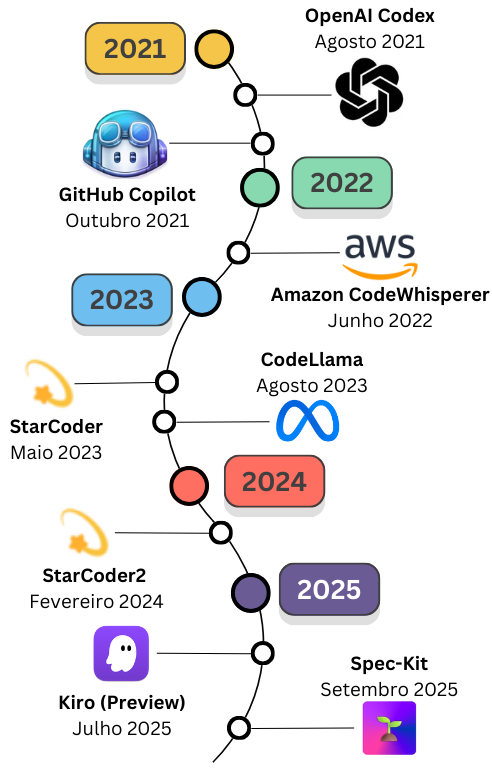
\includegraphics[height=0.3\textheight, width=0.2\textwidth]{../img/code_generation_tineline.png}
    \caption{Linha temporal de alguns dos modelos e ferramentas de geração de código analisados nesta secção.}
    \label{fig:timeline-modelos}
\end{figure}

\subsection{Engenharia de Prompts}

\noindent{Como} já foi referido na secção \ref{PE-BACKGROUND}, a forma como as instruções são fornecidas a um modelo de linguagem tem um impacto direto na qualidade do código que o mesmo consegue gerar. Diversos trabalhos mostram que técnicas de engenharia de prompts podem melhorar significativamente o desempenho em tarefas de linguagem natural para código \cite{ChatGPTGenerationPE,PEIMPACTWITHCODEPROMPTEVAL,PECYCLE}. No resto da secção, são apresentados estudos que aplicam estas técnicas em cenários reais de geração de código, evidenciando a sua importância prática no desenvolvimento de sistemas baseados em LLMs.\\\par


\noindent{Um} dos estudos no contexto da engenharia de prompts aplicada à geração de código é o trabalho de Liu et al.\cite{ChatGPTGenerationPE}, que investiga a forma como diferentes estratégias de prompting influenciam o desempenho do ChatGPT em tarefas de geração de código. Os autores avaliam o modelo no benchmark CodeXGlue, um conjunto de tarefas padronizadas para programação que inclui geração, tradução, refatoração e preenchimento de código, e demonstram que a formulação do prompt tem um impacto substancial na qualidade do código gerado. O estudo aplica técnicas como \textit{chain-of-thought}, instruções comportamentais e otimizações multi-etapa, mostrando que o desempenho do ChatGPT pode melhorar significativamente. Esta conclusão foi alcançada através de métricas como o BLEU que avalia a semelhança entre o código gerado e a solução de referência através da contagem de n-gramas, isto é, sequências contíguas de n tokens que permitem medir a sobreposição entre as duas versões de código e o CodeBLEU, que amplia a abordagem anterior ao incluir informação específica de programas, analisando não apenas n-gramas mas também a estrutura sintática representada por árvores AST e as relações de fluxo de dados.\\\par

\noindent{Adicionalmente} Wang et al.\cite{PET-SELECT}, afirmam que, apesar dos avanços recentes nos LLMs, continua a ser difícil garantir que estes produzam código correto e robusto de forma consistente. Para mitigar este problema, os autores propõem o PET-Select, um método que seleciona automaticamente a técnica de prompting mais adequada com base na complexidade do problema. Avaliado em benchmarks como MBPP e HumanEval, o PET-Select mostrou melhorias moderadas na qualidade do código e reduções significativas no custo de geração, demonstrando que a escolha informada da estratégia de prompting pode ter impacto real no desempenho de modelos orientados à programação.\\\par

\noindent{Um} outro contributo é apresentado por Khojah et al.\cite{PEIMPACTWITHCODEPROMPTEVAL}, que exploraram o impacto de diferentes técnicas de prompt engineering na geração de código. Os autores introduzem o CodePromptEval, um dataset composto por 7072 prompts concebido para avaliar cinco técnicas distintas (few-shot, persona, chain-of-thought, function signature e list of packages) aplicadas à geração de funções completas em 3 modelos, o GPT-4o, Llama 3 e Mistral. O estudo mostra que algumas destas técnicas influenciam de forma significativa a correção e qualidade do código produzido. Contudo, a combinação de várias técnicas não garante necessariamente melhorias adicionais.\\

\noindent{Para} além das técnicas de prompting aplicadas diretamente ao enunciado da tarefa, existe uma linha de investigação que explora estratégias de closed-loop prompting, onde o modelo é instruído a analisar e refinar o próprio código após a primeira geração. Ding et al.\cite{PECYCLE} apresentam o CYCLE, um método que combina geração inicial com iterações sucessivas de auto-refinamento orientadas por feedback, mostrando melhorias na qualidade final do código. De forma complementar, Zhou et al.\cite{PEREFINERCODE} propõem o RefineCoder, que incorpora um mecanismo adaptativo de crítica e correção para permitir que o LLM identifique e ajuste erros no código que produz. Ambos os trabalhos reforçam que a melhoria iterativa guiada pelo próprio modelo pode ser uma alternativa eficaz às abordagens que dependem exclusivamente do prompt inicial, contribuindo para aumentar a fiabilidade do código gerado.
